\section{Case Studies}

To demonstrate the effectiveness of this approach and compare to state of the art existing tools, we describe two case studies.

\subsection{Wheel Brake System}
The Wheel Brake System (WBS) described in AIR6110~\cite{AIR6110} is a well-known example that has been used as a case study for safety analysis, formal verification, and contract based design~\cite{DBLP:conf/cav/BozzanoCPJKPRT15, 10.1007/978-3-319-11936-6-7, CAV2015:BoCiGrMa, Joshi05:SafeComp}. The preliminary work for the safety annex used a simplified model of the WBS~\cite{Stewart17:IMBSA}. In order to demonstrate scalability of our tools and compare results with other studies, we constructed a functionally and structurally equivalent AADL version of one of the most complex WBS NuSMV/xSAP models (arch4wbs) described in~\cite{DBLP:conf/cav/BozzanoCPJKPRT15,mattareiThesis}. We refer readers to this publication for diagrams of the full arch4wbs model~\cite{DBLP:conf/cav/BozzanoCPJKPRT15}. A simplified diagram taken from ARP4761 is shown in Figure~\ref{fig:wbs_arp4761}. 

\begin{figure}[h]
\begin{center}
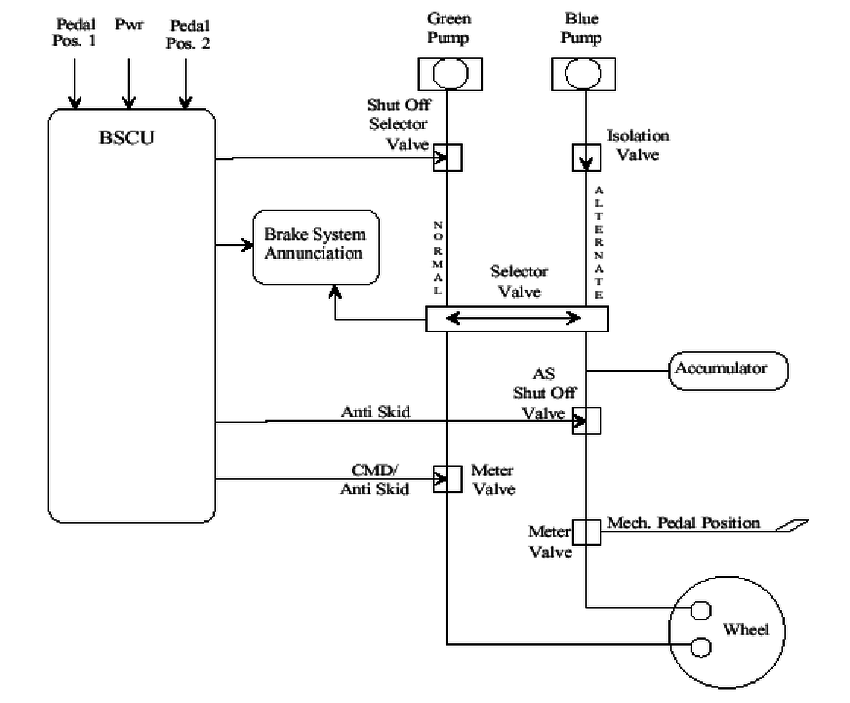
\includegraphics[width=8cm]{images/wbs_arp4761}
\caption{Simplified model of the WBS from ARP4761} \label{fig:wbs_arp4761}
\end{center}
\end{figure}

\subsubsection{WBS architecture description}
The WBS is composed of two main parts: the control system and the physical system. The control system electronically controls the physical system and contains a redundant Braking System Control Unit (BSCU) in case of failure. The physical system consists of the hydraulic circuits running from hydraulic pumps to wheel brakes. This is what provides braking force to each of the 8 wheels of the aircraft.

There are three operating modes in the WBS model. In \textit{normal} mode, the system uses the \textit{green} hydraulic circuit. The normal system is composed of the green hydraulic pump and one meter valve per each of the 8 wheels (shown as one wheel in Figure~\ref{fig:wbs_arp4761}). Each of the 8 meter valves are controlled through electronic commands coming from the BSCU. These signals provide brake commands as well as antiskid commands for each of the wheels. The braking command is determined through a sensor on the pilot pedal position. The antiskid command is calculated based on information regarding ground speed, wheel rolling status, and braking commands.

In \textit{alternate} mode, the system uses the \textit{blue} hydraulic circuit.  The wheels are all mechanically braked in pairs (one pair per landing gear). The alternate system is composed of the blue hydraulic pump, four meter valves, and four antiskid shutoff valves. The meter valves are mechanically commanded through the pilot pedal corresponding to each landing gear. If the system detects lack of pressure in the green circuit, the selector valve switches to the blue circuit. This can occur if there is a lack of pressure from the green hydraulic pump, if the green hydraulic pump circuit fails, or if pressure is cut off by a shutoff valve. If the BSCU channel becomes invalid, the shutoff valve is closed.

The last mode of operation of the WBS is the \textit{emergency} mode. This is supported by the blue circuit but operates if the blue hydraulic pump fails. The accumulator pump has a reserve of pressurized hydraulic fluid and will supply this to the blue circuit in emergency mode.

The model size and statistics are described in Table~\ref{fig:arch_table}. 

\begin{figure}[h]
\begin{center}
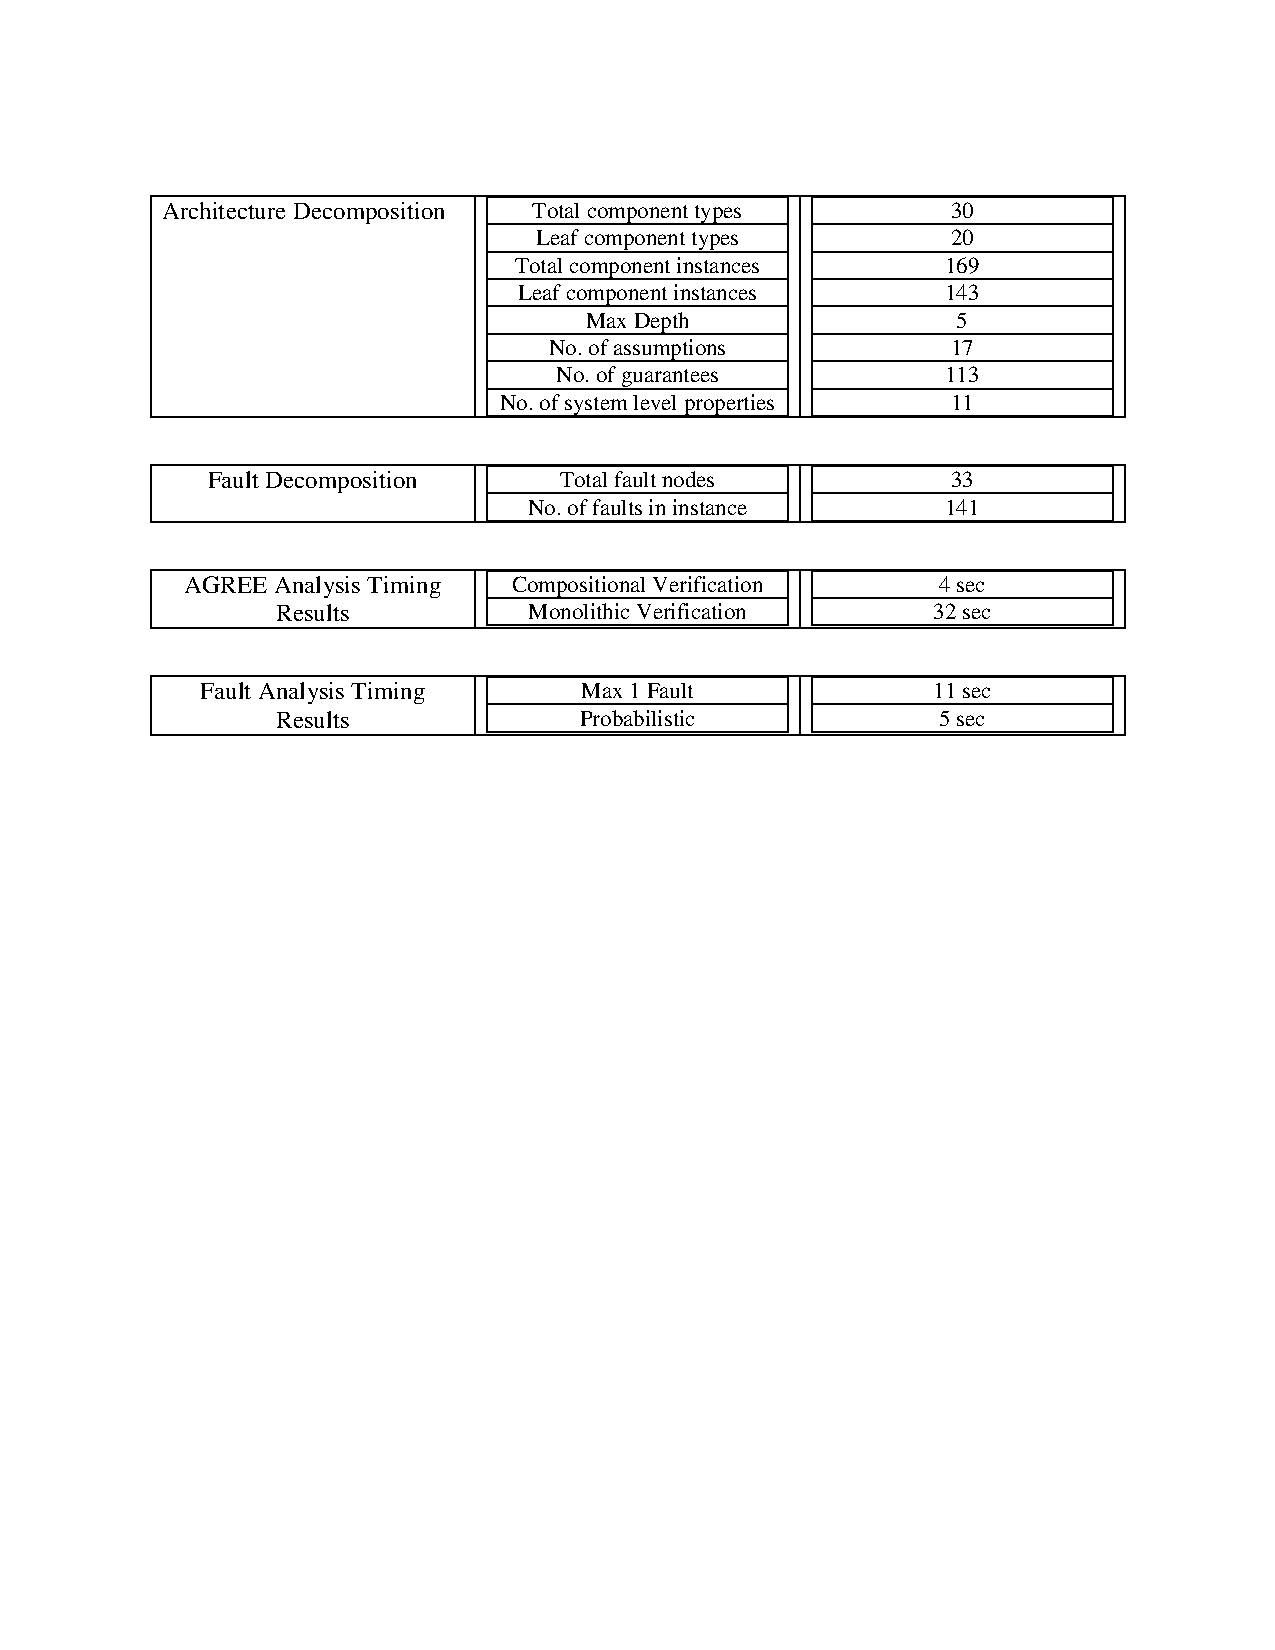
\includegraphics[width=8cm]{images/arch_table.pdf}
\caption{Model Statistics} \label{fig:arch_table}
\end{center}
\end{figure}

\subsubsection{System Safety Properties}
The AIR6110 document contains a set of safety requirements on the expected probability of an unwanted occurance of event, e.g. `'the loss of all wheel braking shall be extremely remote.'' The case study performed using xSAP/NuSMV~\cite{mattareiThesis, DBLP:conf/cav/BozzanoCPJKPRT15} focused on these safety requirements that are outlined in AIR6110. The detailed tech report of the xSAP/NuSMV model of the WBS can be found in~\cite{air6110TechReport}.

\textbf{S18-WBS-R-0321} \textit{Never loss of all wheel braking.}

\textbf{S18-WBS-R-0322-left} \textit{Never asymmetrical loss of wheel braking (left side).}

\textbf{S18-WBS-R-0322-right} \textit{Never asymmetrical loss of wheel braking (right side).}

\textbf{S18-WBS-0323} \textit{Never inadvertent braking with all wheels locked during takeoff roll before V1.}

\textbf{S18-WBS-R-0324} \textit{Never inadvertent braking of all wheels during takeoff roll after V1.}

\textbf{S18-WBS-R-0325-w1...8} \textit{Never inadvertent braking of one wheel without locking (wheels 1-8).} 

\textbf{Braking implies cmd w1...8} \textit{If system is braking, then pilot has commanded braking (wheels 1-8).} 

\textbf{Cmd implies braking w1...8} \textit{If pilot commands braking, then system is braking (wheels 1-8).} 

These requirements violations are the top level events (TLE) for the fault tree computations. 


\subsubsection{Qualitative analysis comparison}
In qualitative analysis, we are interested in the Minimal Cut Sets (MCS), their cardinalities, and the time of computation. Previous work produced hierarchical fault trees for all top level properties without bounds on the cardinality of cut sets or fault restrictions. They performed the hierarchical fault tree generation using OCRA~\cite{6693137} and implemented two procedures to generate the fault trees from the model. the algorithms were either based on existing Binary Decision Diagram (BDD) procedures or a combination of BDD with Bounded Model Checking (BMC). The BMC and BDD approach first computes the MCSs up to some specific depth using BMC and then performs a BDD algorithm to generate the rest of the MCSs. The full description of these procedures and findings can be found here~\cite{10.1007/978-3-319-11936-6-7, mattareiThesis}. 

\subsubsection{Quantitative analysis comparison}
For quantitative analysis, the main calculation of interest is: what is the probability of a TLE occuring? Given a set of MCSs and probabilities for leaf level faults (BEs), the computation of this TLE probability is possible using the techniques described in section III. Previous work has used this technique of TLE probabilistic computation when the MCSs were able to be computed. The TLE probabilities were approximated in the events of timeouts. 
